\minitoc

\vfill

In the previous chapter (Chapter~\ref{chap::semantic_evaluation}), we developped a hierchical and modular taxonomy of errors for the overhead modeling case.
Based on this taxonomy, and depending on the particular needs, specific error labels are extracted and considered during the quality evaluation.\\
In this chapter, we present the second part of our proposed approach.
It is based on formulating the problem as a supervized classification one.
Issues related to the latter are detailed in Section~\ref{sec::learned_evaluation::classification}.
Next, Section~\ref{sec::learned_evaluation::baseline} presents in details the baseline of features extracted out of building \gls{acr::3d} models.
Third and last, richer features are discussed in Section~\ref{sec::learned_evaluation::richer_features}.
These are proposed to better model defect predictions.

\clearpage

\section{\textsc{Quality evaluation as classification}}
    \label{sec::learned_evaluation::classification}
    In order to satisfy the \textbf{large-scale} condition imposed at Subsection~\ref{subsec::introduction::contributions::positioning}, we propose to formulate the problem as a supervized learning one.
    Errors are considered as labels while features are computed so as to describe the observed buildings.
    Actually, as a first approach, the existence of all errors is predicted at the building level, even for \texttt{Facet Errors} labels\footnote{These errors are, in fact, by definition more local.}.
    Determining which facet is affected by an error is a much more challenging problem than the previous one.
    That is why the facet level prediction of errors is not explored in this work.
    The goal is, instead, to test the feasibility of the learning approach.\\

    Errors are predicted based on learned statistical characteristics of the evaluated models.
    The learned approach is usually used to take care of highly semantic tasks, such as ours, that are otherwise hard to process using engineered metrics \addref.\\
    Provided an initial manual annotation effort, the prediction phase is fully automatic, as will be proved by experimental results in Chapter~\ref{chap::experiments}.
    In order for this approach to be scalable at large scales, and hence verify the second constraint in Subsection~\ref{subsec::introduction::contributions::positioning} which is \textbf{automation}, prediction results should be stable enough independently of the urban scene.
    This is fully studied in Chapter~\ref{chap::more_experiments}.\\

    Two aspects should be discussed to in order to apply this approach to the building \gls{acr::3d} model quality evaluation.
    First, as seen in Section~\ref{sec::semantic_evaluation::label_extraction}, the parametric nature of the taxonomy leads to a varying set of labels.
    For this purpose, we describe in Subsection~\ref{subsec::learned_evaluation::classification::different_porblems} the different classification problems depending on the evaluation parameters.
    Second, the feature extraction procedure should also be compliant with the \textbf{large-scale} objective set beforehand.
    This aspect and more are detailed in Section~\ref{subsec::learned_evaluation::classification::feature_extraction}.
    Third, the classifier should be able to handle the heterogeneity of the feature vector and must adapt to different input vectors types and sizes.
    The choice of classifiers is, hence, discussed in Subsection~\ref{subsec::learned_evaluation::classification::classifiers}.

    \subsection{\textsc{Different classification problems}}
        \label{subsec::learned_evaluation::classification::different_porblems}
        The nature of the different classification problems are presented in Table~\ref{tab::classification_problems} depending on the three evaluation parameters defined in Subsection~\ref{sec::semantic_evaluation::label_extraction}.\\

        \begin{table}[htbp]
            \small
            \begin{tabular}{c c c x{11cm}}
                \toprule
                \textbf{\gls{acr::efin}} & \textbf{\gls{acr::elod}} & \textbf{exclusivity} & \textbf{Classification output}\\
                \midrule
                1 & --- & --- & $binary(\texttt{Valid}, \texttt{Erroneous})$\\
                2 & \gls{acr::lod}-1 & --- & $binary(\texttt{Valid}, \texttt{Building Errors})$\\
                2 & \gls{acr::lod}-2 & \textsc{on} & $multi\_class(\texttt{Valid}, \texttt{Building Errors}, \texttt{Facet Errors})$\\
                2 & \gls{acr::lod}-2 & \textsc{off} & $multi\_label(\texttt{Building Errors}, \texttt{Facet Errors})$\\
                3 & \gls{acr::lod}-1 & \textsc{on} & $multi\_stage(\texttt{Valid}, \texttt{Building Errors})$\\
                3 & \gls{acr::lod}-2 & \textsc{on} & $multi\_stage(\texttt{Valid}, \texttt{Building Errors}, \texttt{Facet Errors})$\\
                3 & \gls{acr::lod}-1 & \textsc{off} & $multi\_label(\operatorname{children}(\texttt{Building Errors}))$\\
                3 & \gls{acr::lod}-2 & \textsc{off} & $multi\_label(\operatorname{children}(\texttt{Building Errors})\cup \operatorname{children}(\texttt{Facet Errors}))$\\
                \bottomrule
            \end{tabular}
            \caption{
                \label{tab::classification_problems}
                All possible classification problem types depending of the evaluation parameters:
                \textbf{\gls{acr::efin}}, \textbf{\gls{acr::elod}} and \textbf{exclusivity}.
            }
        \end{table}

        In Table~\ref{tab::classification_problems}, $multi\_class(l_1, l_2, \dots, l_c)$ (\textit{resp.} $multi\_label(l_1, l_2, \dots, l_c)$) corresponds to the multi-class (\textit{resp.} multi-label) setting.
        We note that:
        \begin{equation*}
            multi\_label(\texttt{Valid}, l_1, l_2, \dots, l_c) \equiv multi\_label(l_1, l_2, \dots, l_c).
        \end{equation*}
        $binary$ refers to the special case of $multi\_class$ where $c = 2$: \textit{i.e}
        \begin{equation*}
            binary(l_1, l_2) \equiv multi\_class(l_1, l_2)
        \end{equation*}
        Two consecutive classification problems can be concatenated in a hierchical multi-stage classification:
        depending on the class that is predicted in the first stage multi-class classifier, a second classification problem predicts the existence of some corresponding labels.
        This denoted by:
        \begin{equation*}
            multi\_stage(l_1, l_2, \dots, l_3) \equiv multi\_label(\operatorname{children}(multi\_class(l_1, l_2, \dots, l_3))).
        \end{equation*}
            
        \textbf{\gls{acr::efin}} = 1 level corresponds to the standard binary classification problem: \texttt{Valid} or \texttt{Erroneous}.
        At \textbf{\gls{acr::efin}} = 2, the \textbf{\gls{acr::elod}} can then take two values in the aerial reconstruction case: \gls{acr::lod}-1 or \gls{acr::lod}-2.
        If set at \gls{acr::lod}-1, it is a binary classification problem: \texttt{Valid} or \texttt{Building Errors}.
        For \gls{acr::lod}-2, if the \textbf{exclusivity} is on, it will be a multi-class problem: \texttt{Valid}, \texttt{Building Errors} or \texttt{Facet Errors}.
        If set off, it becomes a multi-label one with the same labels.
        At \textbf{\gls{acr::efin}} = 3 level, if the \textbf{exclusivity} is on, it is a 2-stage classification problem.
        In the first stage, a multi-class task\footnote{It is binary in the spcial case \gls{acr::elod} = \gls{acr::lod}-1, problem, like in the previous semantic degree.}
        predicts the error family, after which a second multi-label problem decides between the predicted error family children.
        If the \textbf{exclusivity} is off, it turns into one stage multi-label problem that predicts the existence of each atomic error corresponding to the chosen \gls{acr::elod}.
    
    \subsection{\textsc{Feature extraction}}
        \label{subsec::learned_evaluation::classification::feature_extraction}
        The proposed quality evaluation approach, being formulated as a supervized classification problem, requires extracting feature vectors describing characteristics of the evaluated model.
        This is possible through the use of the intrinsic properties of the building model, as well as comparisons with external data.\\
    
        Intrinsic feature extraction consists in make use of the geometric structure of the \gls{acr::3d} model.
        Equally, semantics, as well as building model meta-data, could be utilized for the purpose of intrinsically evaluating a model.
        This case corresponds to the minimal amount of information one can use for building model evaluation.
        In this case, we talk about self-evaluation of building models.
        Since we are considering all possible cases, especially automatically reconstructed building models, only the model geometry is guaranteed to be always available.\\
    
        Extrinsic feature extraction relies on comparing the model to an available external data.
        Obviously, high quality reference models are the best type of data to compare the evaluated model to.
        However, taking into consideration the \textbf{large-scale} objective that was fixed earlier (subsection~\ref{subsec::introduction::contributions::use}), this is not a viable solution.
        We rely then on more basic reference data such as remote sensing acquired data that are the basis of large-scale modeling of urban scenes.\\
        For instance, raw depth information can be used in quality evaluation.
        It can prove helpful in detecting geometric defects that are intrinsically of \gls{acr::3d} nature.
        This was illustrated in Figure~\ref{fig::fig}, as comparing the projected model to the orthoimage did not yield anything out of place, contrarily to the \gls{acr::dsm} comparison.
        Depth data can take multiple forms: unstructured point clouds, originating for instance from \gls{acr::lidar} sensors, or dense depth maps such as \gls{acr::dsm} for the overhead case.\\
        Optical images can also be employed in this framework.
        These provide complementary information such as edges (high frequencies, in general) and textures which are suited for inner defect detection as an example (\textit{cf.} Subfigure~\ref{subfig::fus_2d}).
        This type of data comes usually in two different shapes: oblique images or orthoimages.
    
    \subsection{\textsc{Classifier choice}}
        \label{subsec::learned_evaluation::classification::classifiers}
        The choice of classifiers shoud take into consideration the highly modular nature of the framework with multimodal features involving many parameters.
        Two classifiers where chosen in this study: Random Forest and \gls{acr::svm}.
        Both were discussed at great length in Section~\ref{sec::state_of_the_art::mlpr}.
        Hereafter, we explain how each one is used in this setting.\\

        \paragraph{Random Forest}
            Random Forest classifiers is a natural choice in our case.
            As seen in Sub-subsection~\ref{subsubsec::state_of_the_art::mlpr::classifiers::rf}, this type of classifiers can manage a large number of features with different dynamics and coming from multiple modalities.
            In fact, the computed features can be geometric, image based or height based.
            Each one of these modalities can be heterogeneous in terms of extracted value types as will be discussed later in Section~\ref{sec::learned_evaluation::baseline}.
            Relying on their bagging property, a high number of trees is chosen to cover most of the feature space, while a limited tree depth was set to avoid overfitting during training.
            It adapts easily to any of our classification paradigms: multi-class or multi-label.
            The first multi-class case is handled natively by the Random Forest classifier, while for the second one, a one-vs-all approach is adopted so as to address each label separately.

        \paragraph{\acrshort*{acr::svm}}
            \glspl{acr::svm} do not manage heterogeneity in feature vectors and only binary classification is inherently handled.
            However, it offers other advantages that are not met by Random Forest.
            In fact, \glspl{acr::svm} can be useful when labels are not equally distributed in the training set.
            This is actually the case of some errors that are rare in our dataset: specifically the inaccurate topology ones (\textit{cf.} Subsection~\ref{subsec::experiments::datasets::stats}).
            This type of classifiers naturally encorporates kernels such as the ones presented later in Subsection~\ref{subsec::learned_evaluation::richer_features::graph}.
            Finally, it is also preferred when dealing with high dimensional feature vectors like those produced by \glspl{acr::scatnet} (\textit{cf.} Subsection~\ref{subsec::learned_evaluation::richer_features::image}).

\section{\textsc{Feature baseline}}
    \label{sec::learned_evaluation::baseline}
    Since there is no comparable work that studied the learned detection of errors defined in Chapter~\ref{chap::semantic_evaluation}, we propose a baseline for each one of the three modalities: geometric, height based and image based features.
    Attributes are kept simple so as to be used in most situations relying on generally available data.
    We avoid computing and comparing \gls{acr::3d} lines~\parencite{michelin2013quality}, correlation scores~\parencite{boudet2006supervised} or any \gls{acr::sfm} based metric~\parencite{kowdle2011active}.
    In addition of being very costly, these features are methodologically redundant with the \gls{acr::3d} modeling techniques.
    They are, hence, vulnerable to the same defects.
    Conversely, evaluation metrics used in the \gls{acr::3d} building reconstruction literature (\textit{e.g.}, \gls{acr::rmse}) are too weak for such a complex task.
    This will be proven later on in Section~\ref{subsec::experiments::evaluation::feature_analysis}.

    In Subsection~\ref{subsec::learned_evaluation::baseline::geometric}, we describe the used baseline for geometric features.
    Next, in Subsection~\ref{subsec::learned_evaluation::baseline::height}, height based features extraction is explained.
    We end with image based features in Subsection~\ref{subsec::learned_evaluation::baseline::image}.

    \subsection{\textsc{Geometric features}}
        \label{subsec::learned_evaluation::baseline::geometric}
        The model facet set is denoted by $\mathsf{F}$.
        $\forall (f, g) \in \mathsf{F} \times \mathsf{F} \; f \sim g$ correspond to facets $f$ and $g$ being adjacent: 
        \textit{i.e.}, they share a common edge. As the roof topology graph in~\parencite{verma20063d}, the input building model $\mathsf{M}$ can be seen as a facet (dual) graph:

        \begin{equation}
        	\label{eq::model_graph}
        	\mathsf{M} \triangleq \left(\mathsf{F}, \mathsf{E} \triangleq \left\{ \left\{f, g\right\} \subset \mathsf{F} : f \sim g \right\} \right).
        \end{equation}

        \begin{figure}[htbp]
            \centering
            \includestandalone[mode=buildnew, width=.75\textwidth]{figures/features/geometric}
            \caption{
                \label{fig::geometric_features}
                Computed geometric attributes represented on the dual graph, for facets $f$ and $g$.
                The green vector groups the node (facet) attributes while the blue one shows the edge features.
            }
        \end{figure}

        The dual graph is illustrated in Figure~\ref{fig::geometric_features}.
        For each facet $f \in \mathsf{F}$, we compute its degree (\textit{i.e.}, number of vertices; $d(f) \triangleq \left\lvert\left\{v : v\text{ is a vertex of }f\right\}\right\rvert$), its area $\mathscr{A}(f)$ and its circumference $\mathscr{C}(f)$.
        These are all geometric invariants with respect to $\mathbb{R}^3$ isometries, contrarily to facet centroids $\mathscr{G}(f)$ and normals $\vec{n}(f)$.
        This is countersteped by looking, for each graph edge $e=\left\{f, g\right\} \in \mathsf{E}$, for the distance between facet centroids $\Vert \mathscr{G}(f) - \mathscr{G}(g) \Vert$ and the angle formed by their normals $\arccos(\vec{n}(f) \cdot \vec{n}(g))$.
        Statistical characteristics are then computed over building model facets using specific functions $S$, like a histogram:        

        \begin{equation}
            \label{eq::histogram_extractor}
        	S = S^p_{\text{histogram}}: l \mapsto \operatorname{histogram}(l, p),
        \end{equation}
        with $p$ standing for histogram parameters. A simpler option could be:
        \begin{equation}
            \label{eq::statistical_extractor}
            S = S_{\text{manual}}: l \mapsto \begin{bmatrix}
                \max(l)\\
                \min(l)\\
                \operatorname{mean}(l)\\
                \operatorname{median}(l)\\
                \sigma(l)
            \end{bmatrix},
        \end{equation}
        where:
        \begin{conditions}
            \sigma(l) & represents the standard deviation over samples $l$.
        \end{conditions}

        These features are designed for general topological errors.
        For instance, over-segmentation may result in small facet areas and small angles between their normals.
        Conversely, an undersegmented facet would have a large area.
        Later on, the importance of these features will be discussed in details based on experimental results.
        
        Each building $\mathsf{M}$ can consequently be characterized by a geometric feature vector that accounts for its geometric characteristics:

        \begin{equation}
        	\label{eq::geometric_features}
            v_{\text{geometry}}(\mathsf{M}) = \begin{bmatrix}
            	S \Big(\big(d(f)\big)_{f \in \mathsf{F}}\Big)\\
                S \Big(\big(\mathscr{A}(f)\big)_{f \in \mathsf{F}}\Big)\\
                S \Big(\big(\mathscr{C}(f)\big)_{f \in \mathsf{F}}\Big)\\
                S \Big(\big( \vert\vert \mathscr{G}(f) - \mathscr{G}(g) \vert\vert \big)_{(f,g) \in \mathsf{E}}\Big)\\
                S\Big(\big( \arccos(\vec{n}(f) \cdot \vec{n}(g)) \big)_{(f,g) \in \mathsf{E}}\Big)
            \end{bmatrix}.
        \end{equation}

        Additionally to individual facet statistics, regularity is taken into account by looking into adjacent graph nodes as in~\parencite{zhou20102}.
        Such features express a limited  part of structural information.
        Dealing with this type of information implies graph comparisons which are not a genuinely simple task to achieve.
        Since our objective is to build a baseline, this approach has not yet been considered.

    \subsection{\textsc{Height based features}}
        \label{subsec::learned_evaluation::baseline::height}
        For this modality, raw depth information is provided by a \gls{acr::dsm} as a \gls{acr::2d} height grid: $dsm \in \mathbb{R}^{w\times h}$\footnote{$w$ (\textit{resp.} $h$) is the grid width (\textit{resp.} height)}.
        This type of reference data must date back to the same time where the building models where produced.
        Otherwise a lot of defects will result simply from change in the scenery.\\

        The \gls{acr::dsm} is compared to the model height~\parencite{bredif20073d,zebedin2008fusion}.
        The latter is inferred from its facets plane equations.
        It is rasterized into an grid structure $alt \in \mathbb{R}^{w\times h}$ using the same spatial resolution as $dsm$.
        The difference between the two height grids provides a discrepancy map (Figure~\ref{fig::height_based_features}.c).
        A baseline approach is herein proposed relying on the statistics of pixel values computed using the $S$ functions (Figure~\ref{fig::height_based_features}).

        \begin{equation}
            \label{eq::height_based_features}
            v_{\text{height}}\left(\mathsf{M}\right) = S\left( dsm - alt \right).
        \end{equation}
        
        \begin{figure}[htpb]
            \centering
            \includestandalone[width=\textwidth, mode=buildnew]{figures/features/height_based}
            \caption{
                \label{fig::height_based_features}
                Height-based features computed from the \gls{acr::dsm} residuals using histograms.
            }
        \end{figure}

        Equation~\ref{eq::height_based_features} summarizes how building height-based features are computed.
        Different from a \gls{acr::rmse}~\parencite{lafarge2012creating,poullis2013framework}, the histogram captures the discrepancy distribution, which is particularly helpful in detecting undersegmentation defects or geometric imprecision.
        However, as for the previous geometric attributes, the grid structure information coming from the model is lost.
        Errors cannot be spatialized and linked to a specific facet.

    \subsection{\textsc{Image based features}}
        \label{subsec::learned_evaluation::baseline::image}
        The framework is general enough to encompass both orthorectified images and oblique ones.
        For now, we rely only on more accessible orthorectified images, eventhough they can be riddled with artifacts.
        In an ideal scenario, using oriented images is better for edge verification (as already shown in~\parencite{michelin2013quality}) as orthoimages are a byproduct of earlier ones.
        However, in practice, oblique imagery would give rise to other issues, especially, registration problems.\\

        We aim to benefit from the high frequencies in Very High Spatial Resolution optical images.
        Building edges, like any image edge, correspond to sharp discontinuities in images~\parencite{ortner2007building}.
        The latter are detected using gradient filters on images.
        Gradient based features are advantageous compared to any radiometry based ones.
        This is due to the fact that the latter are much less invariant to changes in the than the first ones.
        Indeed, classic Computer Vision techniques rely on gradient based features:~\textcite{lowe2004distinctive,dalal2005histograms}.
        This is adequate to our case where models and images are part of large heterogeneous datasets.\\
        

        We apply this to our context by comparing these edges to local gradients.
        We start by projecting building models on the orthorectified image $I$ (Figure~\ref{subfig::model_nadir_projection}).
        For each facet, we isolate an edge $s$ (Figure~\ref{subfig::segment_gradient_collinearity}).
        In an ideal setting, gradients computed at pixels $g$ that intersect $s$ need to be almost be collinear with its normal $\vec{n}(s)$.
        In consequence, applying the same statistics functions $S$, we compute the distribution of the cosine similarity between the local gradient and the normal all along that $s$:
        
        \begin{equation}
            \label{eq::corr_seg}
            \mathsf{D}_S(s, I) \triangleq S \left( \left(\frac{\nabla I(g) \cdot \vec{n}(s)}{\left\rVert \nabla I(g)\right\rVert}\right)_{\substack{g \in I \\ g \cap s \neq \emptyset}} \right).
        \end{equation}

        \begin{figure}[htpb]
            \begin{center}
                \floatbox{figure}{
                    \begin{subfloatrow}[2]
                        \ffigbox[\FBwidth]{
                            \caption{
                                Model facets (each represented by a specific color) are nadir projected onto the orthoimage.
                            }\label{subfig::model_nadir_projection}
                            }			
                            {
                                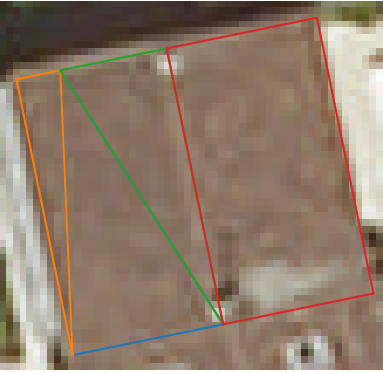
\includegraphics[width=.45\textwidth]{images/features/image/nadir_superposition}
                            }
                        \quad
                        \ffigbox[\FBwidth]{
                                \caption{Local gradients (in purple), on intersecting pixels (in green), are compared to the edge (in red) normal (in black).}
                                \label{subfig::segment_gradient_collinearity}
                            }
                            {\includestandalone[mode=buildnew, width=.45\textwidth]{figures/features/radiometric_features}
                        }
                    \end{subfloatrow}
                }{
                    \caption{Illustration of how features are derived from optical images.}\label{fig::image_based}
                }
            \end{center}
        \end{figure}

        Once the distribution is computed over a segment, it is stacked over all facet edges to define the distribution over projected facets.
        In the case of histograms $S^p_{\text{histogram}}$ with the same parameters (and thus the same bins), it is equivalent to summing out the previous vectors $\mathsf{D}_{S^p_{\text{histogram}}}(s, I)$ over edges $s$ from the projection $q(f)$ of the facet $f$.
        In order to take into account the variability of segment dimensions, this sum is normalized by segment lengths.

        \begin{equation}
            \label{eq::corr_fac}
            D_{S^p_{\text{histogram}}}\left(f, I\right) \triangleq \sum_{s \in q(f)} \left\rVert s \right\lVert \cdot \mathsf{D}_{S^p_{\text{histogram}}}(s, I).
        \end{equation}

        The same can be done over all facets of a building $\mathsf{M}$ (Equation~\ref{eq::corr_bul}).
        The weights are added in order to take into account the geometry heterogeneity.
        The gradient to normal comparison is similar to the \gls{acr::3d} data fitting term formulated in~\parencite{li2016manhattan}.
        Once again, the model structure is partially lost when simply summing histograms over all segments.

        \begin{equation}
            \label{eq::corr_bul}
            v_{\text{image}}\left(\mathsf{M}\right) = D_{S^p_{\text{histogram}}}\left(\mathsf{M}, I\right) \triangleq \sum_{f \in \mathsf{F}} \mathscr{A}\left(q(f)\right) \cdot \mathsf{D}_{S^p_{\text{histogram}}}(f, I).
        \end{equation}
        
        These image-based attributes are helpful for precision error detection.
        As example, facet imprecise borders can be detected as local gradients direction will be expected to differ greatly from the inaccurate edge.
        It can also be detrimental in under-segmentation detection as colors can change considerably from one facet or one building to another inducing an gradient orthogonal to edge normals.

\section{\textsc{Richer features}}
    \label{sec::learned_evaluation::richer_features}
    \subsection{\textsc{Graph classification}}
        \label{subsec::learned_evaluation::richer_features::graph}
        

    \subsection{\textsc{Image classification}}
        \label{subsec::learned_evaluation::richer_features::image}
